\subsection{Hyperledger Composer}
\label{sec:prototype_composer}
        Hyperledger Composer\cite{ComposerDocs} ist eine Abstraktion des Hyperledger Fabric Frameworks und dient vornehmlich für das Entwickeln von Blockchain-Netzwerken. 
        \medskip\\
        Composer bietet die Möglichkeit private Blockchainnetzwerke, genannt ,,Business Networks``, zu entwickeln und innerhalb eines Docker-Container zu betreiben.
        Weitere Werkzeuge des Frameworks können eine konfigurierbare \gls{rest}-\gls{api} und eine minimalistische Angular-Webapplikation generieren.
        \medskip\\
        Für die Entwicklung der Transaktionslogik von Business Networks wird die Sprache JavaScript verwendet. 
        Darüber hinaus werden domainspezifische Sprachen jeweils für die Modellierung der Teilnehmer im Netzwerk, sowie der Zugriffskontrolle und Anfragen and die Blockchain eingesetzt.
        \medskip\\
        Alle erfolgreichen Transaktionen von Assets werden im Ledger, gespeichert, wobei der aktuelle World State zusätzlich in einer Datenbank gespeichert wird. 
        Das Framework sorgt dafür, dass der Ledger und die Datenbank an alle Knoten verteilt wird und konsistent bleibt.\\
        Der ,,Historian`` schreibt zusätzlich alle weiteren Transaktionen wie das Hinzufügen oder Entfernen eines Teilnehmers in \colorbox{light-gray}{\lstinline{Historian Records}}, einem speziellen Typ von Asset, das ebenfalls in der Blockchain gespeichert wird.
        
        \subsubsection*{Aufbau}
            Ein Business Network besteht aus Assets, Participants, Transactions, \gls{acl}, optionalen Events und optionalen Queries.
            \begin{itemize}
                \item \textsc{Assets}: matrielle oder immatrielle Güter, die auf der Blockchain gespeichert werden
                \item \textsc{Participants}: Teilnehmer des Netzwerkes, kann Assets besitzen und Transaktionen einreichen
                \item \textsc{Transactions}: Funktionen, die ausgeführt werden können, können Smart Contracts (sogenannte ,,Transaction Processor Functions``) auslösen, die  beliebige Aktionen ausführen können
                \item \textsc{Access Control Rules}: legen fest, welche Teilnehmer welche Aktionen im Netzwerk ausüben dürfen. 
                    Zu vergebende Berechtigungen bestehen grundlegend aus einer Operation (CRUD\!\footnote{Create, Read, Update, Delete}), der betroffenen Ressource (Asset, Participant oder Transaction) und dem Akteur, der die Operation ausführt.
                    Die Regeln werden sequentiell in geordneter Reihenfolge ausgewertet. 
                \item \textsc{Events}: können während der Transaktionsverarbeitung generiert werden und dafür genutzt werden externe Systeme von Ereignissen in der Blockchain zu benachrichtigen, sofern sie die Events abonniert haben
                \item \textsc{Queries}: ähnlich wie Anfragen an eine Datenbank, können mit Queries Daten aus der Blockchain gelesen und beispielsweise automatisch weiterverarbeitet werden
            \end{itemize}
            Die einzelnen Bestandteile werden zu einem ,,Business Network Archive`` zusammengefasst und auf einer Hyperledger Fabric-Instanz ausgerollt (siehe \fref{fig:composer_arch}).
            
            \begin{figure}[H]
        		\centering
        		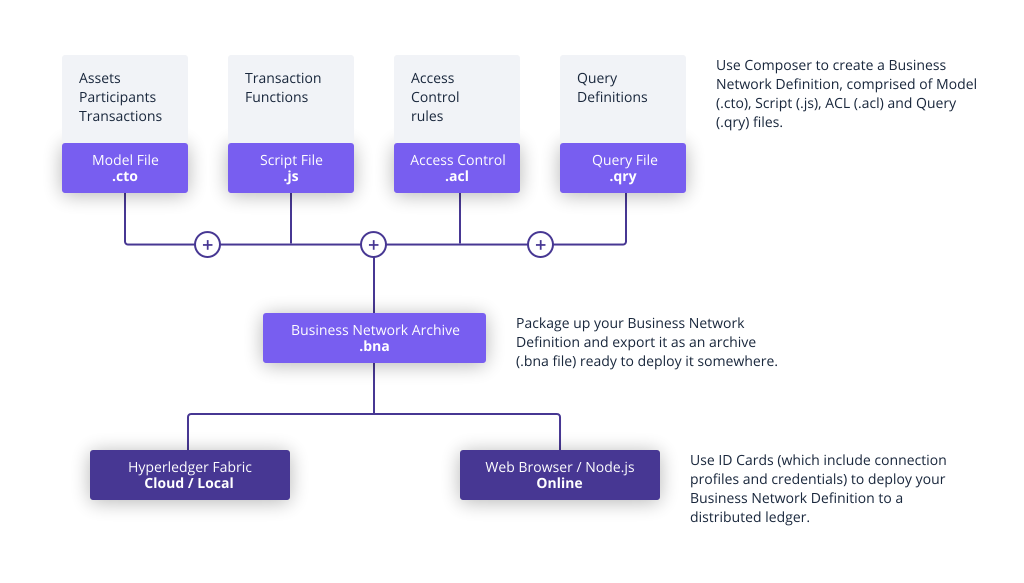
\includegraphics[width=0.8\textwidth]{graphics/Composer-Diagram.png}
        		\caption[Zusammensetzung einer Hyperledger Composer-Applikation]{Zusammensetzung einer Hyperledger Composer-Applikation\cite{ComposerDocs}}
        		\label{fig:composer_arch}
        	\end{figure}
        
        \subsubsection*{Identitäten}
            Eine Identität ist ein digitales Zertifikat und ein privater Schlüssel.
            Sie wird dazu genutzt am Netzwerk teilzunehmen und müssen pro Identität einem Participant zugeordnet sein.
            Ein Participant-Typ kann jedoch einer oder mehreren Identitäten zugeordnet werden.
            
        \subsubsection*{Administration}
            Im Kontext des Frameworks existieren zwei Arten von Administratoren: Ein PeerAdmin undn ein Business Network Adminstrator.\\
            Ein PeerAdmin ist für die jeweilige lokale Hyperledger Instanz verantwortlich, stellt, falls noch nicht vorhanden, die Identität für den Business Network Administrator aus und kann diese auch wieder entziehen. 
            Ebenfalls ist ein PeerAdmin dafür verantwortlich ein Business Network auf dessen Knoten initial auszurollen.
            Es ist möglich, dass ein PeerAdmin auch mehrere verschiedene Business Networks auf dem selben Knoten verwaltet.\\
            Der Business Network Administrator existiert einmal pro Business Network und verwaltet dieses.
            Zu dessen Aufgaben gehören Updates des Netzwerks (z.B. eine neue Art von Transaktionen wird eingeführt), sowie die Identitätsverwaltung der Participants
